\chapter{Desarrollo del Experimento}
En este capítulo se detalla el proceso explicado en el capítulo anterior para cada actividad de la metodología aplicada, así como los entregables comprometidas.

\section{Comprensión del negocio}
\textbf{Actividad 1: Definir problemas, objetivos e hipótesis}
\\
El inicio de la implementación de la primera fase de la metodología CRISP-DM fue la identificación del problema general a partir del estudio de la realidad problemática abordada en los primeros capítulos. El objetivo, por lo tanto, busca resolver el problema y se encuentra alineado con el título de la investigación. Asimismo, la hipótesis resulta la proposición planteada para explicar el logro del objetivo. Los objetivos específicos del trabajo, que responde a cada problema específico, se definieron a partir de una lluvia de ideas en base a la asociación de objetivos específicos de los antecedentes con la actual investigación. Estos se explican en la siguiente actividad.

\textbf{Actividad 2: Desarrollar la literatura de la investigación}
\\
Se buscaron desde libros y artículos online para la comprensión teórica del financiamiento colectivo e Inteligencia Artificial, hasta papers publicados en conferencias, revistas internacionales y científicas, reportes técnicos y tesis de grado acerca de propuestas para resolver el problema estudiado en la investigación.

Para ello, como se describió en la sección 3.2, a través de búsqueda de palabras clave como \textit{crowdfunding}, \textit{Machine Learning}, \textit{Deep Learning}, \textit{prediction}, \textit{Kickstarter}, \textit{accuracy} y \textit{projects}, y el uso del buscador Google Académico, se encontraron estos papers publicados entre el 2013 y 2020.

A continuación, se realizó un resumen de cada antecedente en una hoja de cálculo de Excel con el fin de comparar sus objetivos y metodologías implementadas, como se puede observar el detalle en el Anexo \ref{anexo5}.

\textbf{Actividad 3: Definir metodología de la investigación}
\\
Luego de elaborar el detalle del anterior anexo, a excepción de la investigación del autor \cite{pr_fernandezblanco2020crowdfunding_empirical} que utilizó la metodología CRISP-DM, cada antecedente fue agrupado con otro similar de acuerdo a los pasos seguidos en su propia metodología. El resultado fue la Tabla \ref{2:table1} explicada en la sección 3.3.1.

\section{Comprensión de los datos}
\textbf{Actividad 1: Construir base de datos de Metainformación}
\\
El punto de partida para la construcción de los conjuntos de datos que se usaron más adelante en cada modelo de acuerdo a su modalidad fue la adquisición de bases de datos capturadas mensualmente desde finales del 2015 hasta 2019 por la página Web Robots (\url{https://webrobots.io/kickstarter-datasets/}), fundada por los ex corporativos de TI Tomás Vitulskis y Paulius Jonaitis, como se aprecia en la Figura \ref{4:fig1} \cite{ot_webrobots2019kickstarter}. Para el presente trabajo, se optó por descargar en archivos de valores separados por comas (.csv). De acuerdo sus creadores, se ejecutan robots en dos servidores en la nube encargados de recolectar en un determinado punto del día y una vez al mes información de las campañas que aparecen en Kickstarter.

\begin{figure}[!ht]
	\begin{center}
		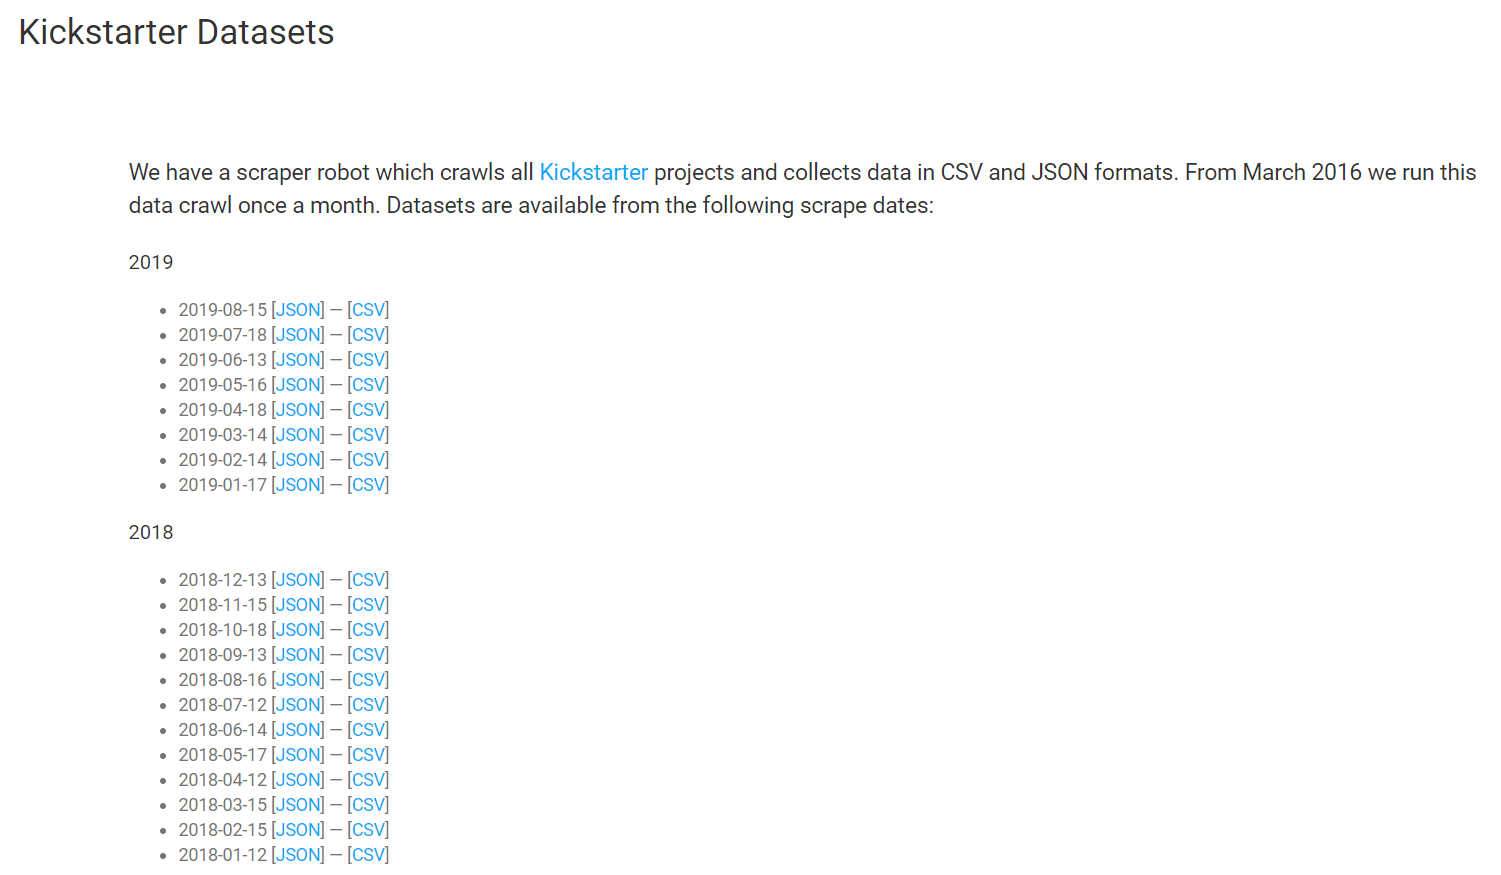
\includegraphics[width=1\textwidth]{4/figures/web_robots_2019.png}
		\caption[Vista del website Web Robots (visitado en agosto del 2019)]{Vista del website Web Robots (visitado en agosto del 2019).\\
		Fuente: Elaboración propia.}
		\label{4:fig1}
	\end{center}
\end{figure}

A continuación, los archivos descargados que se encontraban fraccionados en varios archivos .csv, donde luego de ser descomprimidos, fueron unidos por mes de captura y almacenados en carpetas independientes por mes, cuyo peso individual osciló entre 1 y 5 gigabytes (GB). Con el fin de ahorrar espacio en la computadora, las partes originales fueron eliminadas.

En la Figura \ref{4:fig2} se detalla el tamaño del conjunto de datos total al corte del periodo de captura de información Julio 2019, aproximadamente más de 212 mil proyectos de todas las categorías y 37 columnas de variables.

\begin{figure}[h]
	\begin{center}
		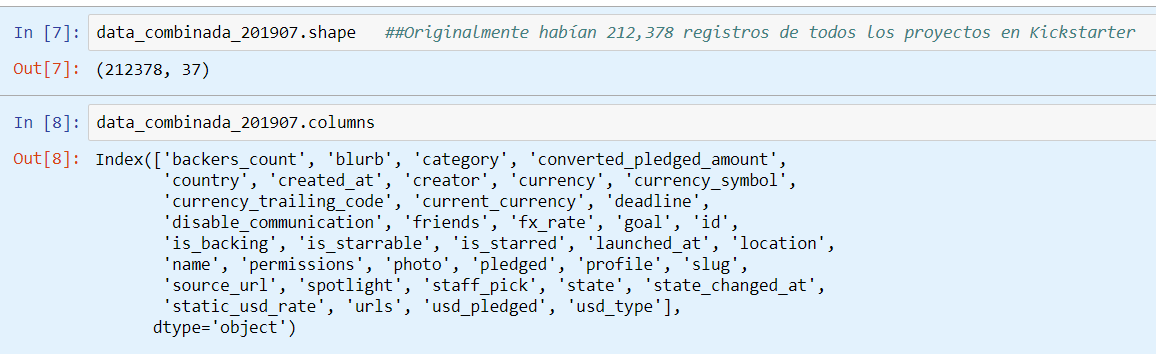
\includegraphics[width=1\textwidth]{4/figures/dataset_201907.png}
		\caption[Tamaño de conjunto de datos al corte de Julio 2019]{Tamaño de conjunto de datos al corte de Julio 2019.\\
			Fuente: Elaboración propia.}
		\label{4:fig2}
	\end{center}
\end{figure}

A cada conjunto de datos generado se filtraron los que pertenecen a la categoría \textit{\textbf{Technology}}. Al no contar con la información de la columna \textit{main\_category}, este proceso se logró utilizando la variable \textit{source\_url} seleccionando aquellos registros que contengan la cadena de caracteres “\textbf{https://www.kickstarter.com/discover/categories/technology}”.

Cuando se repitió este procedimiento con cada conjunto generado, se observó que la proporción de proyectos tecnológicos en Kickstarter representa el 10\% de la totalidad, aproximadamente más de 21 mil registros por mes. Esto se calculó al comparar el tamaño de cada conjunto generado con el total.

A continuación, se unieron los 45 archivos separados por coma (.csv) capturados mensualmente desde noviembre del 2015 hasta agosto del 2019. Se realizaron 2 uniones internamente ya que, a partir de marzo del 2018, algunas de las variables y valores presentan diferente estructura a la de sus predecesoras.

Luego, se realizó limpieza de datos para las variables \textit{category}, \textit{location}, \textit{photo} y \textit{urls}, y se transformaron las variables numéricas en milisegundos \textit{created\_at}, \textit{launched\_at} y \textit{deadline} a variables de fecha. Esto último permitió calcular la variable \textit{duration} para determinar la duración de la campaña (en días) de un proyecto calculando la diferencia entre la fecha de culminación (\textit{deadline}) y la fecha de lanzamiento (\textit{launched\_at}). Luego se excluyeron los proyectos en proceso de la variable \textit{state} para conservar los culminados, es decir, aquellos cuyo valor sea “successful” o “failed” ya que se analizarán solamente los proyectos que han sido exitosos o fracasados. Los proyectos cancelados o suspendidos no aparecieron. El último paso del flujo consistió en generar y exportar el archivo final en formato .csv. En la Figura \ref{4:fig4} se visualiza el conjunto final de Metainformación subido públicamente a la plataforma Kaggle. Cada variable se detalla en la Tabla \ref{4:table1}.

\begin{figure}[h]
	\begin{center}
		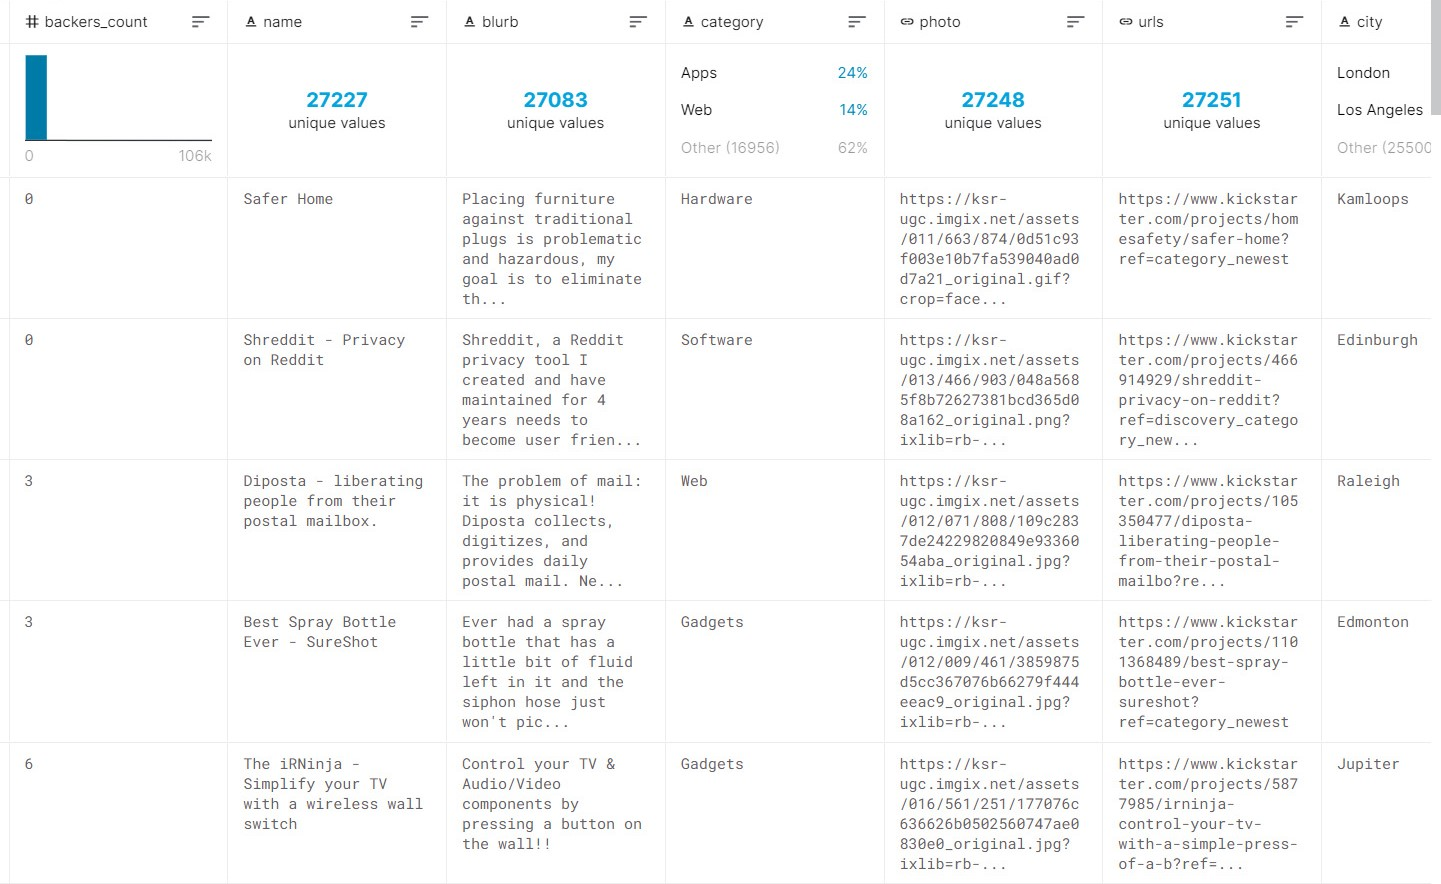
\includegraphics[width=0.93\textwidth]{4/figures/metadata_kaggle_preview.jpg}
		\caption[Visualización del archivo de metainformación subido a Kaggle]{Visualización del archivo de metainformación subido a Kaggle.\\
			Fuente: Elaboración propia.}
		\label{4:fig4}
	\end{center}
\end{figure}

\begin{table}[h!]
	\caption[Diccionario de datos del dataset final de Metainformación]{Diccionario de datos del dataset final de Metainformación.}
	\label{4:table1}
	\centering
	\small
	\begin{tabular}{ m{3cm}m{9.5cm}m{2.5cm} }
		\specialrule{.1em}{.05em}{.05em}
		\Centering{Variable}& \Centering{Detalle}& \Centering{Tipo de dato}\\
		\specialrule{.1em}{.05em}{.05em}
		id & Identificador del proyecto. & number \\
		%\hline
		backers\_count & Número de patrocinadores de la campaña del proyecto. & number \\
		%\hline
		name &	Nombre del proyecto. &	string \\
		%\hline
		blurb & Propaganda del proyecto. & string \\
		%\hline
		category & Categoría (dentro de categoría principal) del proyecto. & string \\
		%\hline
		photo & Dirección de enlace de la foto del proyecto. & string \\
		%\hline
		urls & Dirección de la página de la campaña del proyecto. & string \\
		%\hline
		city & Ciudad del creador del proyecto. & string \\
		%\hline
		country & Código de país del creador del proyecto. & string \\
		%\hline
		goal &	Monto de la meta de financiamiento del proyecto. &	float \\
		%\hline
		pledge\_amounts & Montos disponibles para patrocinar la campaña. & string \\
		%\hline
		pledged & Monto final patrocinado de la campaña. & float \\
		%\hline
		currency & Divisa del monto final patrocinado. & string \\
		%\hline
		usd\_pledged & Monto final patrocinado de la campaña (en USD). & float \\
		%\hline
		created\_at & Fecha de creación de la campaña. & date \\
		%\hline
		launched\_at & Fecha de lanzamiento de la campaña. & date \\
		%\hline
		deadline & Fecha de culminación de la campaña. & date \\
		%\hline
		duration &	Duración de la campaña (en días). &	number \\
		%\hline
		state & Estado de financiamiento del proyecto. & string \\
		\specialrule{.1em}{.05em}{.05em}
	\end{tabular}
	%\par	%%Salto de linea
	%\bigskip
	\begin{flushleft}	%%Alinear a la izquierda sin justificar
		\small Fuente: Elaboración propia.
	\end{flushleft}
\end{table}

\newpage
\textbf{Actividad 2: Construir base de datos de Descripción}
\\
La variable \textit{description} se obtuvo utilizando web scraping en cada proyecto gracias a la variable \textit{urls}. Para ello, se elaboró un algoritmo usando la librería BeautifulSoup que, mediante acceso y navegación al contenido de estas páginas a través de un agente falso, se dirigió a las descripciones de los proyectos identificando las etiquetas con clase llamada “\textbf{rte\_\_content js-full-description responsive-media}” y las almacenó en un vector vacío, uniendo previamente todos los párrafos y eliminando caracteres especiales, para posteriormente asignarle la id de su proyecto y guardarlo en un archivo de extensión .csv y exportarlo. En caso el algoritmo no encuentre esta clase dentro de las páginas (\textit{IndexError}), el vector almacena con el valor “null”.

\begin{figure}[!ht]
	\begin{center}
		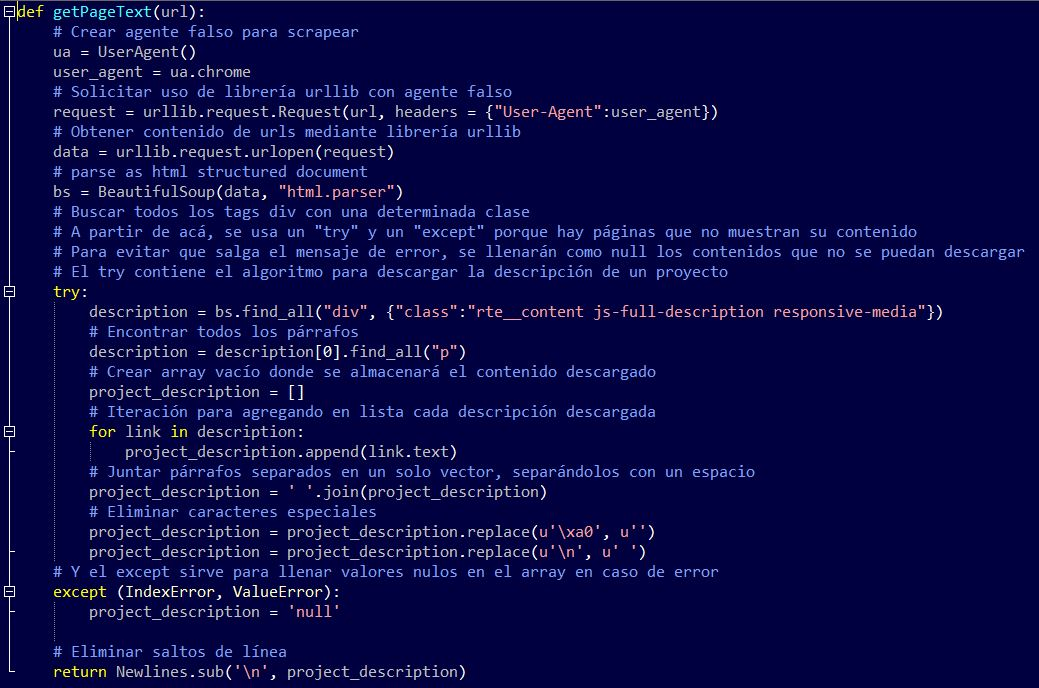
\includegraphics[width=1\textwidth]{4/figures/description_scraping.jpg}
		\caption[Función para extraer textos de modalidad de descripción]{Función para extraer textos de modalidad de descripción.\\
			Fuente: Elaboración propia.}
		\label{4:fig5}
	\end{center}
\end{figure}

Debido a la gran cantidad de memoria y tiempo que iba a presentar este proceso, se determinó fraccionar los 27,251 proyectos en tres partes y repetir el mismo en cada uno de ellos. El tiempo aproximado de descarga de cada fracción fue de 6 horas.

Finalmente, las tres partes fueron unidas, se reemplazaron los valores nulos por espacios en blanco y se guardó como un nuevo archivo de valores separados por coma (.csv) en código Unicode UTF-8 para la lectura de caracteres no alfabéticos, como se observa en la Figura \ref{4:fig6}.

\begin{figure}[!ht]
	\begin{center}
		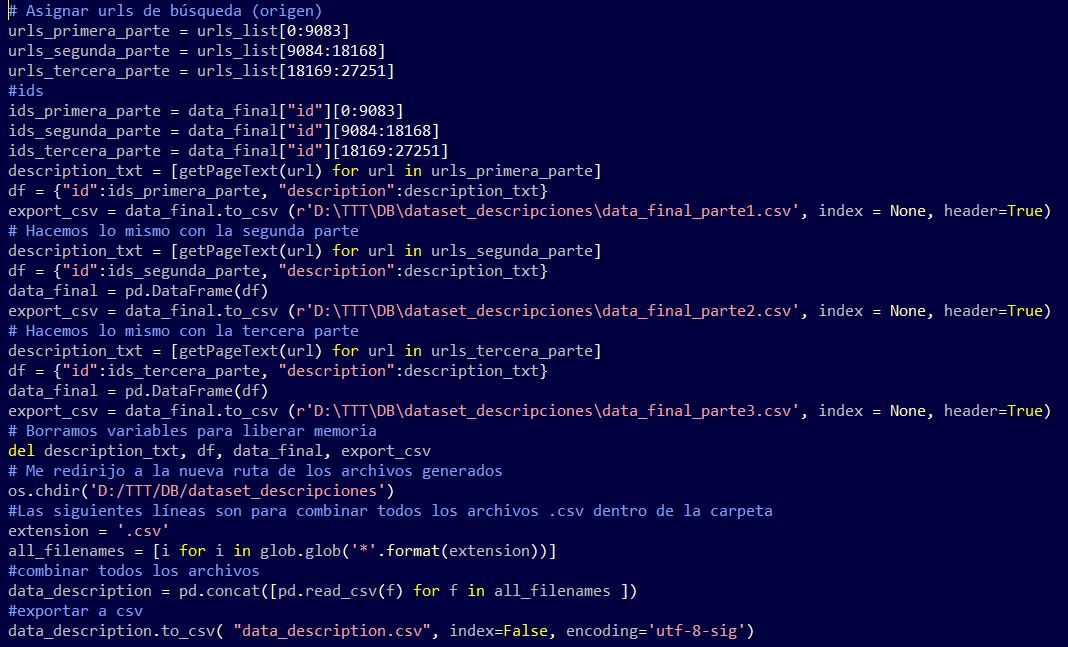
\includegraphics[width=0.95\textwidth]{4/figures/description_scraping_execution.jpg}
		\caption[Ejecución de la función de extracción de descripciones y almacenamiento]{Ejecución de la función de extracción de descripciones y almacenamiento.\\
			Fuente: Elaboración propia.}
		\label{4:fig6}
	\end{center}
\end{figure}

El archivo generado fue subido a la plataforma Kaggle de manera pública para que pueda ser descargada a través del API de la web, como se aprecia en la Figura \ref{4:fig7}.

\begin{figure}[!ht]
	\begin{center}
		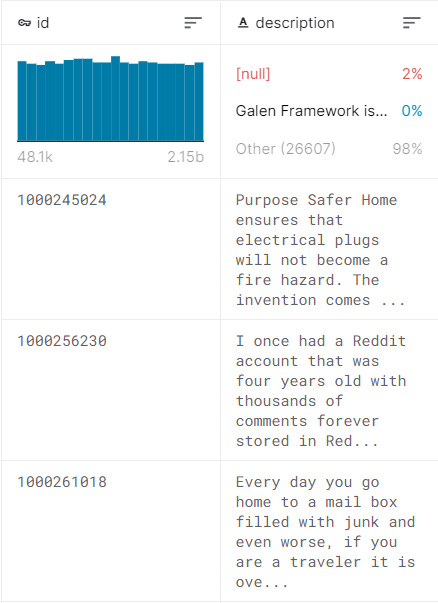
\includegraphics[width=0.36\textwidth]{4/figures/description_kaggle_preview.jpg}
		\caption[Visualización del archivo de descripción subido a Kaggle]{Visualización del archivo de descripción subido a Kaggle.\\
			Fuente: Elaboración propia.}
		\label{4:fig7}
	\end{center}
\end{figure}

\textbf{Actividad 3: Construir base de datos de Comentarios}
\\
Al igual que la descripción, los comentarios se obtuvieron utilizando la variable \textit{urls} para web scraping, pero reemplazando caracteres que contengan desde “\textbf{?ref=}” en adelante, por “\textbf{/comments}” para redireccionarse a la sección de comentarios de cada proyecto. Para lograrlo, se codificó la función de la Figura \ref{4:fig8}.

\begin{figure}[!ht]
	\begin{center}
		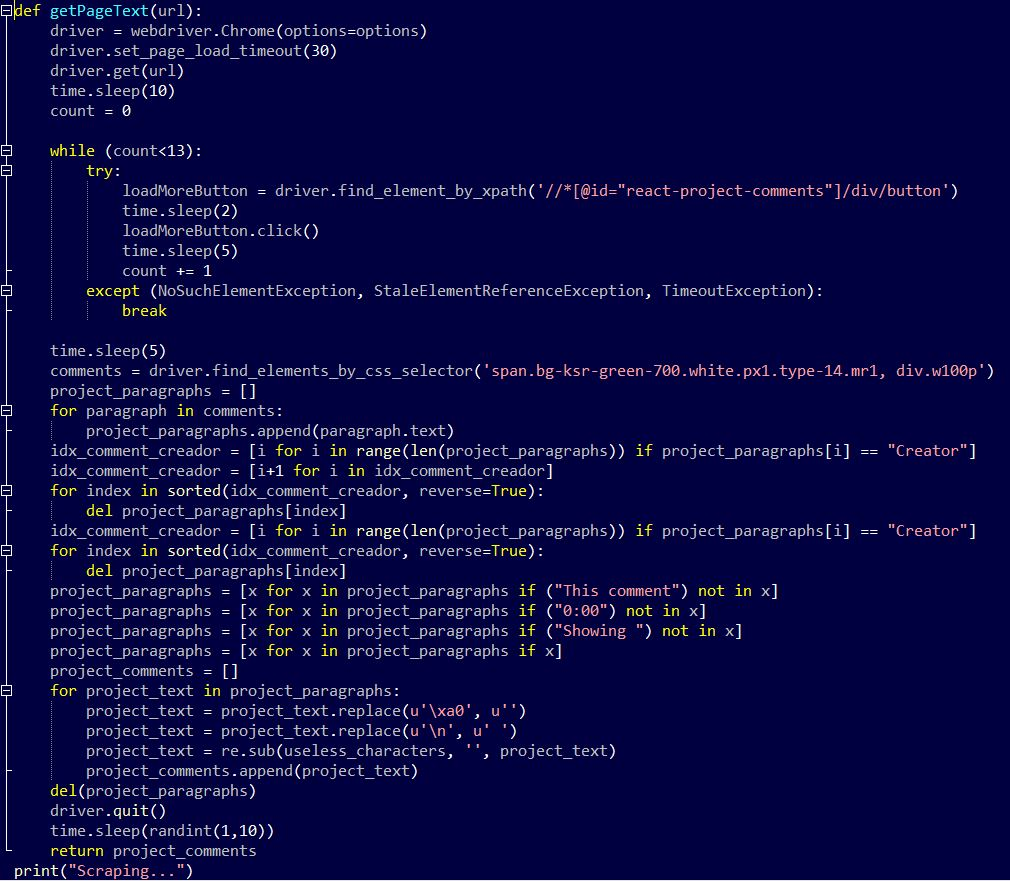
\includegraphics[width=1\textwidth]{4/figures/comments_scraping.jpg}
		\caption[Función para extraer textos de modalidad de comentarios]{Función para extraer textos de modalidad de comentarios.\\
			Fuente: Elaboración propia.}
		\label{4:fig8}
	\end{center}
\end{figure}

Los comentarios, al ser dinámicos, no podían ser extraídos mediante la librería BeautifulSoup como en el caso de las descripciones, por lo que se utilizó la librería Selenium para extraerlos al iniciar una sesión desde Google Chrome. Una vez permitido el acceso al navegador, el algoritmo se redirecciona a la sección de comentarios del proyecto, espera un máximo de 30 segundos de carga de la página, busca el elemento Xpath “\textbf{//*[@id="react-project-comments"]/div/button}” para hacer clic en el botón “Load More” (Cargar más) hasta un máximo de 13 veces esperando 2 segundos entre cada clic, busca todos los comentarios bajo el nombre del elemento CSS “\textbf{div.w100p}”, elimina aquellos que pertenezcan al creador del proyecto identificados con etiqueta verde en el extremo superior derecho del recuadro del comentario con el nombre del elemento “\textbf{span.bg-ksr-green-700.white.px1.type-14.mr1}” (asignados con el valor de «Creator»), y almacena los restantes que pertenecen a los patrocinadores. En caso no encuentre ningún item de comentarios en la sección, se asignará un valor aleatorio no relacionado con proyectos. Luego de eliminar mensajes de la página acerca de comentarios ocultos o eliminados, el algoritmo culmina creando la lista de comentarios separados por autor y cerrando el web driver. Esta función fue ejecutada en 16 partes, asignando el id respectivo a los comentarios extraídos por cada proyecto en un archivo .csv, como se observa en la Figura \ref{4:fig9}.

\begin{figure}[!ht]
	\begin{center}
		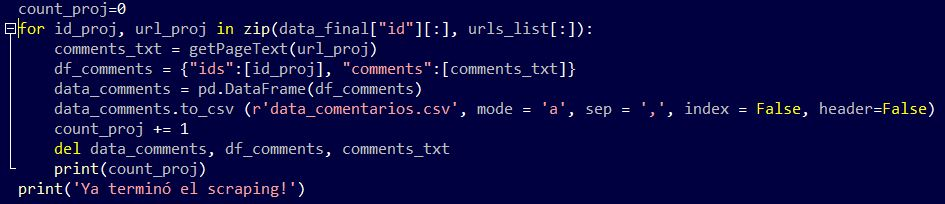
\includegraphics[width=1\textwidth]{4/figures/comments_scraping_execution.jpg}
		\caption[Ejecución de la función de extracción de comentarios y almacenamiento]{Ejecución de la función de extracción de comentarios y almacenamiento.\\
			Fuente: Elaboración propia.}
		\label{4:fig9}
	\end{center}
\end{figure}

Para optimizar la descarga, se crearon 8 instancias en Google Cloud (Figura \ref{4:fig10}).

\begin{figure}[!ht]
	\begin{center}
		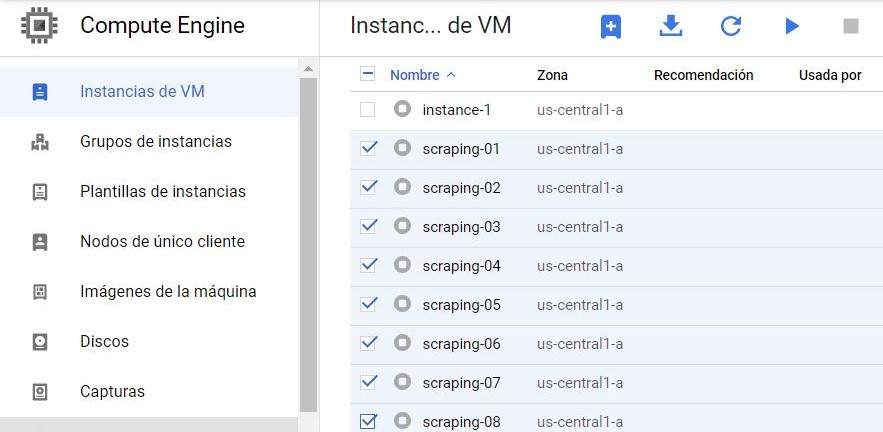
\includegraphics[width=0.95\textwidth]{4/figures/gc_instances_comments.jpg}
		\caption[Instancias lanzadas en paralelo para la extracción de comentarios]{Instancias lanzadas en paralelo para la extracción de comentarios.\\
			Fuente: Elaboración propia.}
		\label{4:fig10}
	\end{center}
\end{figure}

Cada instancia contenía dos copias del algoritmo, con la cantidad de proyectos fraccionada en 16 partes para que sean ejecutados en paralelo. Si bien el tiempo total de la consolidación de esta base de información duró aproximadamente un mes debido a percances de la conexión interna de las instancias y algunos problemas de ineficiencia de la primera versión del algoritmo, durante el transcurso dentro de este lapso de tiempo fueron solucionados hasta lograr optimizar el algoritmo de web scraping y tener el conjunto final de datos tomó menos de 48 horas. Este se encuentra disponible públicamente en Kaggle y se visualiza en la Figura \ref{4:fig11}.

\begin{figure}[!ht]
	\begin{center}
		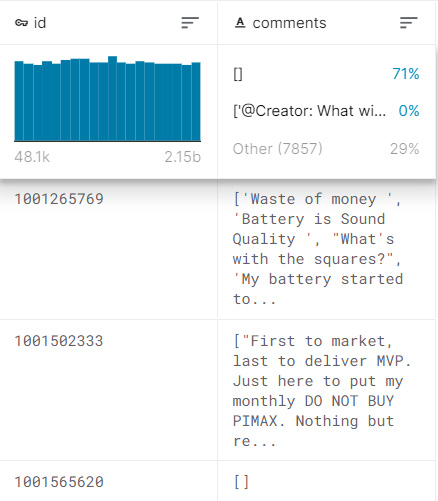
\includegraphics[width=0.43\textwidth]{4/figures/comments_kaggle_preview.jpg}
		\caption[Visualización del archivo de comentarios subido a Kaggle]{Visualización del archivo de comentarios subido a Kaggle.\\
			Fuente: Elaboración propia.}
		\label{4:fig11}
	\end{center}
\end{figure}

\textbf{Actividad 4: Realizar análisis exploratorio y estadístico de variables considerados}
\\
En esta sección, se analizaron estadísticamente las variables de cada modalidad, tanto las distribuciones de sus datos para la metainformación y contenido textual, así como estadísticos para las variables cuantitativas de la metainformación, entre ellos el rango de sus valores, la media, la mediana, la moda, la desviación estándar y la varianza. En la variable dependiente estado de financiamiento, los 27,251 proyectos se distribuyen mediante el gráfico de pie de la Figura \ref{4:fig12}. Se observa que casi 20 mil proyectos entre 2009 y 2019 no llegaron a ser financiados, es decir, aproximadamente el 72\% del total fracasaron.

\begin{figure}[!ht]
	\begin{center}
		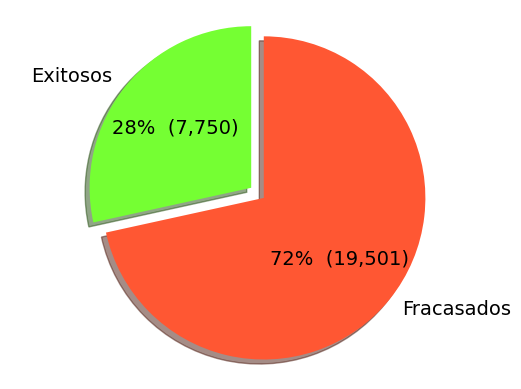
\includegraphics[width=0.60\textwidth]{4/figures/projects by state.png}
		\caption[Distribución de proyectos tecnológicos según su estado]{Distribución de proyectos tecnológicos según su estado.\\
			Fuente: Elaboración propia.}
		\label{4:fig12}
	\end{center}
\end{figure}

\newpage
De acuerdo a la distribución por año de la Figura \ref{4:fig13}, 2015 fue el periodo en donde se registraron más campañas de proyectos tecnológicos en la plataforma.

\begin{figure}[!ht]
	\begin{center}
		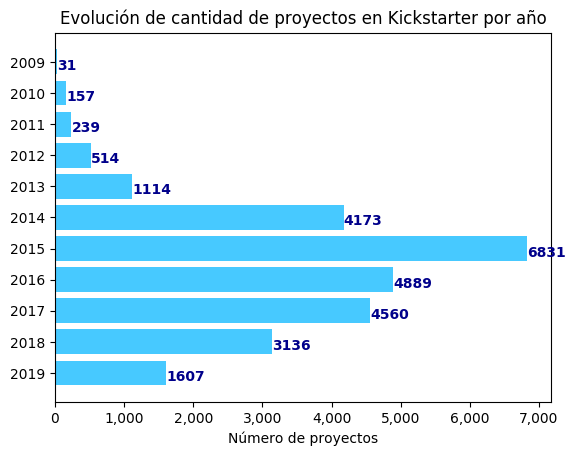
\includegraphics[width=0.77\textwidth]{4/figures/projects state by year.png}
		\caption[Evolución de cantidad de proyectos tecnológicos por año]{Evolución de cantidad de proyectos tecnológicos por año.\\
			Fuente: Elaboración propia.}
		\label{4:fig13}
	\end{center}
\end{figure}

El anterior gráfico abierto por estado de financiamiento, como se representa en la Figura \ref{4:fig14}, muestra que el 2015 resultó ser el año más disparejo, donde el 78\% fueron fracasados.

\begin{figure}[!ht]
	\begin{center}
		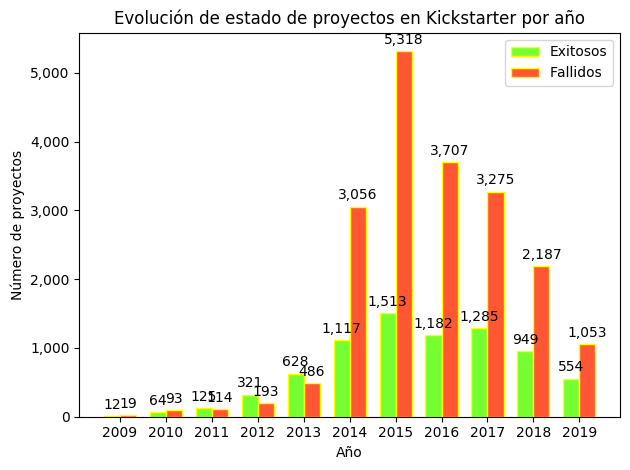
\includegraphics[width=0.77\textwidth]{4/figures/projects state evolution by year.png}
		\caption[Evolución de proyectos tecnológicos, por su estado y año]{Evolución de proyectos tecnológicos, por su estado y año.\\
			Fuente: Elaboración propia.}
		\label{4:fig14}
	\end{center}
\end{figure}

Por el lado de Metainformación, de las 19 variables de la Tabla \ref{4:table1}, se consideraron como potenciales variables independientes a 3 categóricas, 5 numéricas y 1 lista compuesta por números (\textit{pledge\_amounts}). La distribución del primer grupo se ilustra en la Figura \ref{4:fig15}.

\begin{figure}[!ht]
	\centering
	\small
	\begin{subfigure}{.35\textwidth}
		\centering
		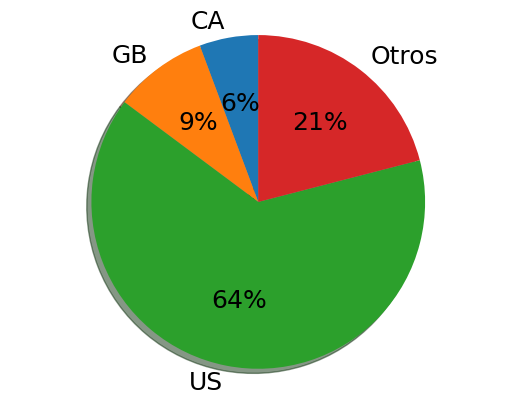
\includegraphics[width=1.13\linewidth]{4/figures/country_distribution.png}
		\caption{país}
	\end{subfigure}%
	\begin{subfigure}{.36\textwidth}
		\centering
		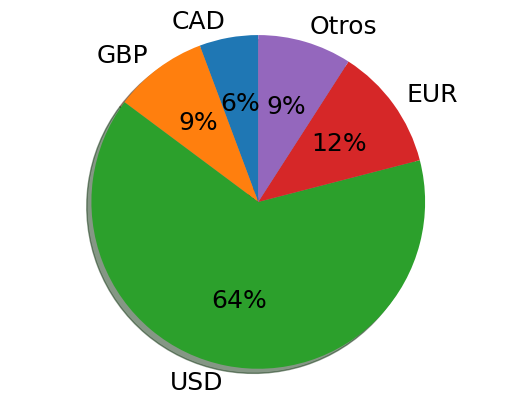
\includegraphics[width=1.13\linewidth]{4/figures/currency_distribution.png}
		\caption{divisa}
	\end{subfigure}%
	\begin{subfigure}{.35\textwidth}
		\centering
		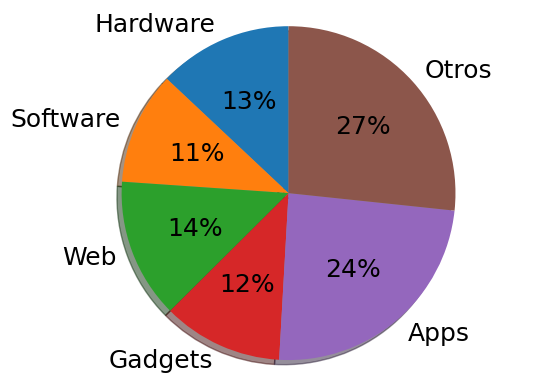
\includegraphics[width=1.15\linewidth]{4/figures/category_distribution.png}
		\caption{categoría}
	\end{subfigure}
	\caption[Distribución de las variables categóricas de Metainformación]{Distribución de las variables categóricas de Metainformación.\\
		Fuente: Elaboración propia.}
	\label{4:fig15}
\end{figure}

De las 3 variables categóricas (\textit{country}, \textit{currency} y \textit{category}), se observa que más de la mitad de creadores proyectos provienen de los Estados Unidos (64\%) e invierten en dólares. A ellos los acompañan personas de Gran Bretaña (9\%), que invierten en libras esterlinas, y de Canadá (6\%), que invierten en dólares canadienses. El 21\% restante provienen de otros países, donde el 12\% de ellos invierten en euros. Por el lado de las categorías, las más resaltantes son Apps, Web, Hardware, Software y Gadgets.

Para las potenciales variables numéricas de Metainformación (\textit{backers\_count}, \textit{goal}, \textit{pledged}, \textit{usd\_pledged} y \textit{duration}), se calcularon sus datos estadísticos de rango de valores, media, mediana, desviación estándar y varianza, con ayuda de diagramas de caja y bigote que se muestran a continuación:

\begin{itemize}
	\item Número de patrocinadores de la campaña (\textit{backers\_count}):
	\begin{itemize}
		\item Rango de valores: [0; 105,857]
		\item Media: 208.710469340575
		\item Mediana: 9.487
		\item Desviación estándar: 1,179.68237749203
		\item Varianza: 1,391,650.51176525
		\begin{figure}[!ht]
			\begin{center}
				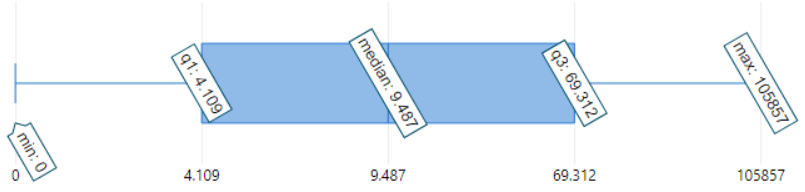
\includegraphics[width=0.80\textwidth]{4/figures/caja_bigote_backers.png}
				\caption[Diagrama de caja y bigote de patrocinadores]{Diagrama de caja y bigote de patrocinadores.\\
					Fuente: Elaboración propia.}
				\label{4:fig16}
			\end{center}
		\end{figure}
	\end{itemize}
	\item Monto meta de la campaña (\textit{goal}):
	\begin{itemize}
		\item Rango de valores: [1; 100,000,000]
		\item Media: 91,263.9666162825
		\item Mediana: 15,762.614
		\item Desviación estándar: 1,259,282.1587922
		\item Varianza: 1,585,791,555,452.35
		\begin{figure}[!ht]
			\begin{center}
				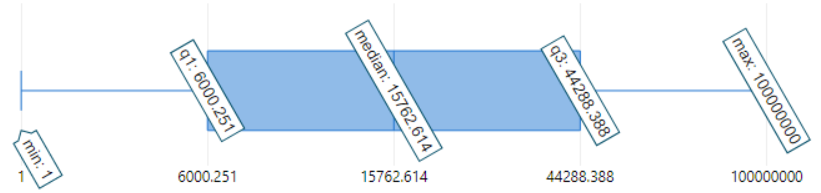
\includegraphics[width=0.80\textwidth]{4/figures/caja_bigote_goal.png}
				\caption[Diagrama de caja y bigote de meta]{Diagrama de caja y bigote de meta.\\
					Fuente: Elaboración propia.}
				\label{4:fig17}
			\end{center}
		\end{figure}
	\end{itemize}
	\item Monto patrocinado al final de la campaña (\textit{pledged}):
	\begin{itemize}
		\item Rango de valores: [0; 17,406,300]
		\item Media: 34,668.5134710787
		\item Mediana: 1,382.933
		\item Desviación estándar: 226,763.900313481
		\item Varianza: 51,421,866,485.3822
		\begin{figure}[!ht]
			\begin{center}
				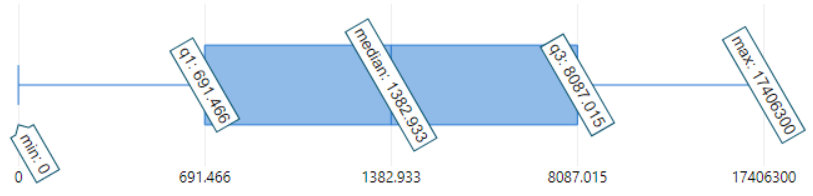
\includegraphics[width=0.80\textwidth]{4/figures/caja_bigote_pledged.png}
				\caption[Diagrama de caja y bigote de monto patrocinado]{Diagrama de caja y bigote de monto patrocinado.\\
					Fuente: Elaboración propia.}
				\label{4:fig18}
			\end{center}
		\end{figure}
	\end{itemize}
	\item Duración de la campaña (\textit{duration}).
	\begin{itemize}
		\item Rango de valores: [1; 92]
		\item Media: 35.4654141132436
		\item Mediana: 30
		\item Desviación estándar: 11.84570862999998
		\item Varianza: 140.320812946853
		\begin{figure}[!ht]
			\begin{center}
				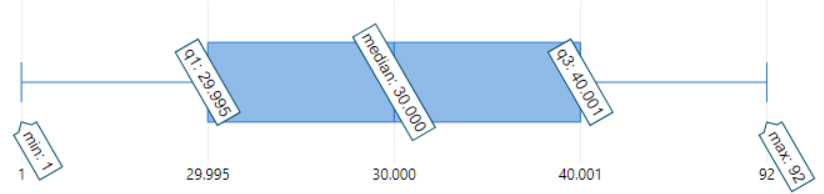
\includegraphics[width=0.80\textwidth]{4/figures/caja_bigote_duration.png}
				\caption[Diagrama de caja y bigote de duración]{Diagrama de caja y bigote de duración.\\
					Fuente: Elaboración propia.}
				\label{4:fig19}
			\end{center}
		\end{figure}
	\end{itemize}
\end{itemize}

\newpage
Posterior a este entendimiento de datos, se elaboró una matriz de correlaciones (Figura \ref{4:fig20}) para encontrar correlaciones entre ellas y determinar la existencia de alguna variable redundante y descartarla para no afectar el rendimiento del modelo.

\begin{figure}[!ht]
	\begin{center}
		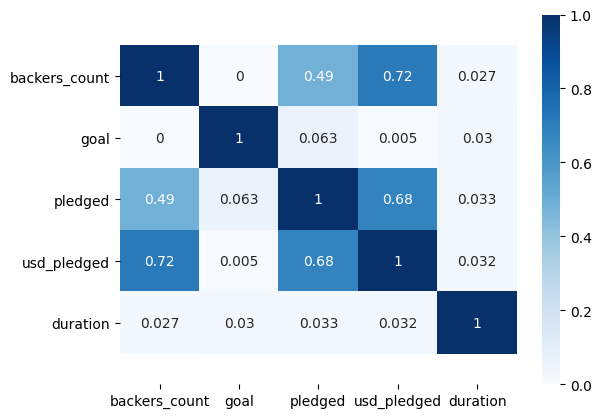
\includegraphics[width=0.90\textwidth]{4/figures/metadata correlation.png}
		\caption[Matriz de correlaciones entre variables independientes]{Matriz de correlaciones entre variables independientes.\\
			Fuente: Elaboración propia.}
		\label{4:fig20}
	\end{center}
\end{figure}

Como se puede apreciar en la figura anterior, la variable \textit{usd\_pledged} está altamente correlacionada con las variables \textit{backers\_count} y \textit{pledged} (ambas con un aproximado de 70\%). Esto quiere decir que dicha variable no es significativa porque explicaría de manera muy similar a las otras dos.

\newpage
Asimismo, si se observan los registros desde una matriz que contiene, además de gráficos de dispersión de las correlaciones, histogramas de las variables independientes como en la Figura \ref{4:fig21}, se confirma y concluye no utilizar las observaciones comentadas.

\begin{figure}[!ht]
	\begin{center}
		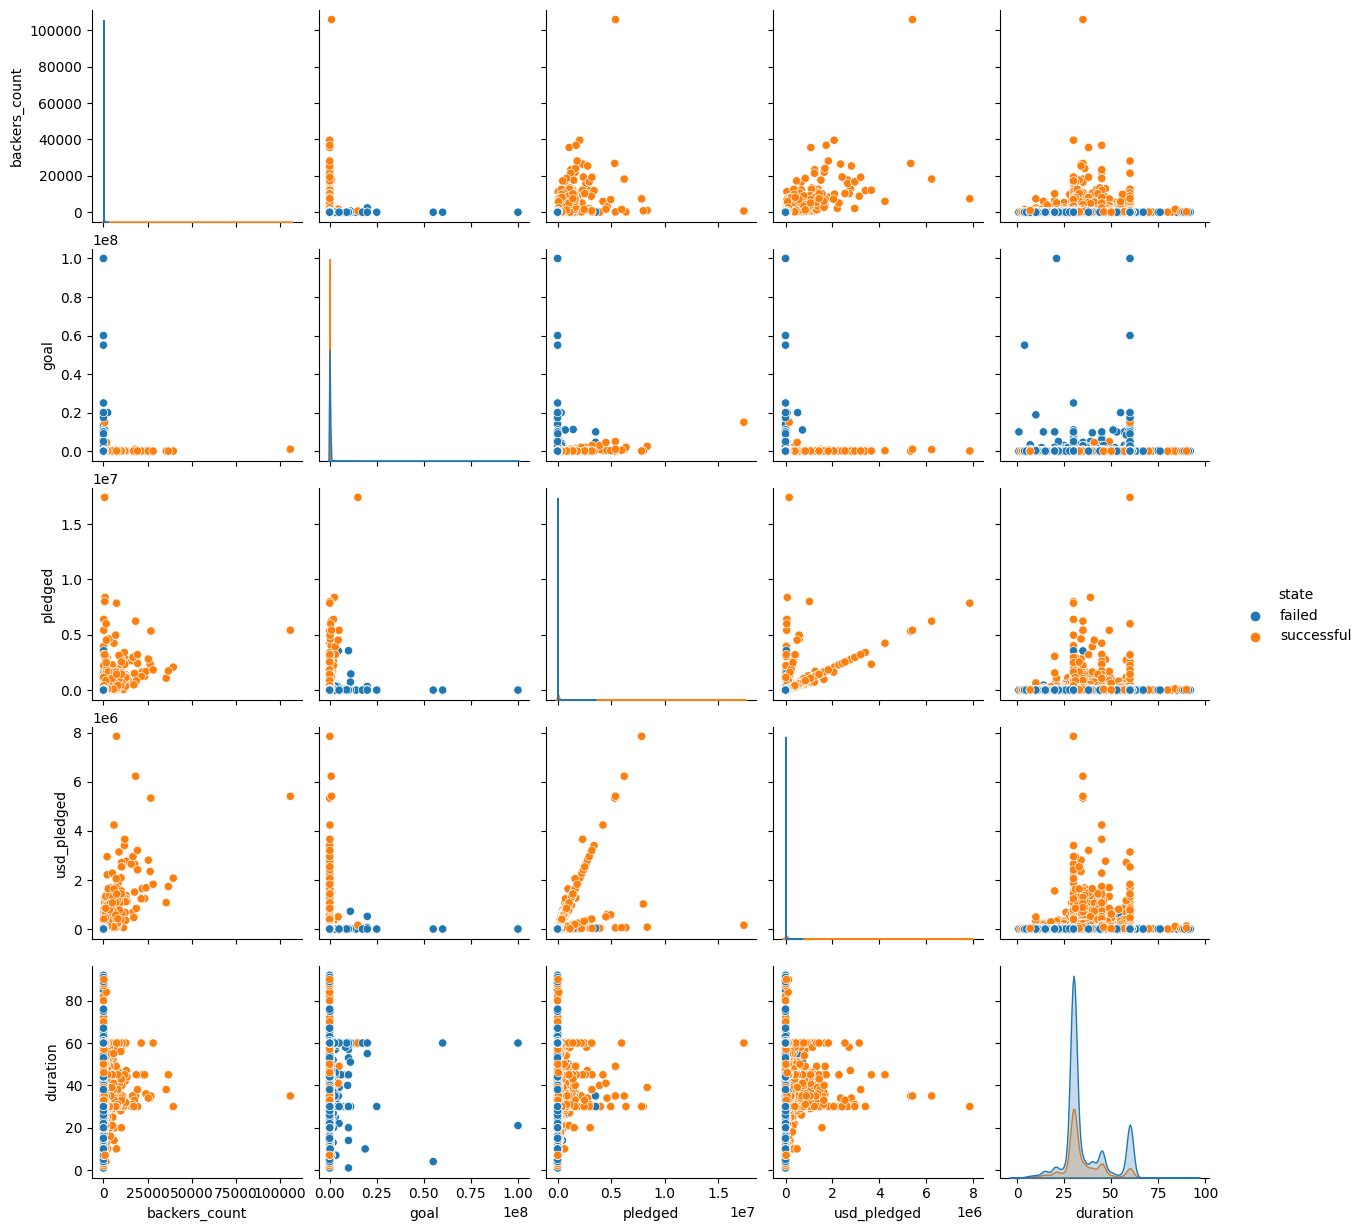
\includegraphics[width=1.00\textwidth]{4/figures/metadata cor-plot2.png}
		\caption[Gráfico de dispersión de correlaciones entre variables independientes]{Gráfico de dispersión de correlaciones entre variables independientes.\\
			Fuente: Elaboración propia.}
		\label{4:fig21}
	\end{center}
\end{figure}

La variable \textit{duration} es la única que sigue una distribución normal debido a la forma de campana de su silueta. Asimismo, los registros de proyectos exitosos y fracasados para las otras 4 variables se encuentran mezcladas en los mismos grupos al cruzarse entre ellas. También se visualizan observaciones en los extremos de cada gráfico, tal y como se detalló en sus valores estadísticos individuales.

\newpage
Por el lado de Descripción, solo 640 proyectos (2\% del total) no presentaron descripciones por razones externas durante el proceso de extracción de datos. De ellos, 512 (80\% de proyectos sin descripciones) fracasaron en ser financiados. Por el lado de proyectos con descripciones, casi el 30\% fueron exitosos como se grafica en la Figura \ref{4:fig22}.

\begin{figure}[!ht]
	\begin{center}
		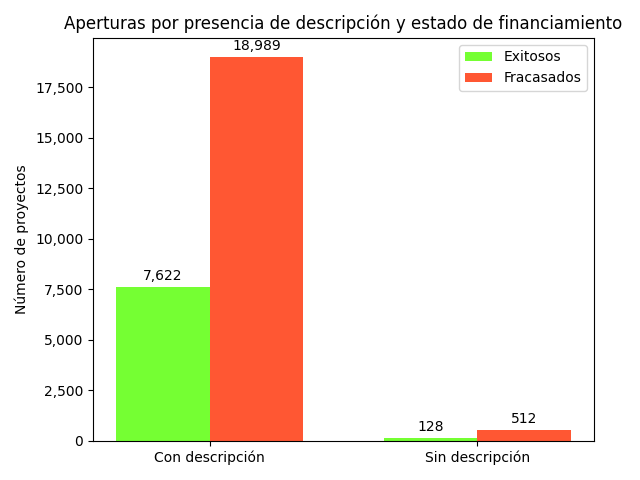
\includegraphics[width=0.75\textwidth]{4/figures/projects description by state.png}
		\caption[Distribución de proyectos por presencia de descripciones y estado final]{Distribución de proyectos por presencia de descripciones y estado final.\\
			Fuente: Elaboración propia.}
		\label{4:fig22}
	\end{center}
\end{figure}

Asimismo, el registro con descripción de mayor longitud presentó 5,152 palabras y, a nivel total de proyectos, el vocabulario fue de 165,683 palabras.

\begin{figure}[!ht]
	\begin{center}
		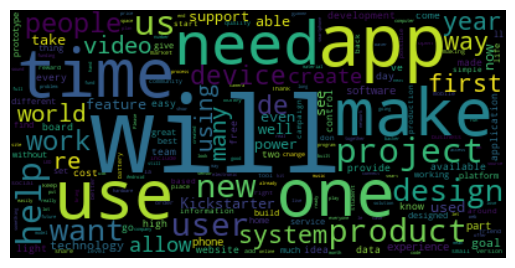
\includegraphics[width=0.64\textwidth]{4/figures/description_wordcloud_original_data.png}
		\caption[Nube de palabras de descripciones]{Nube de palabras de descripciones.\\
			Fuente: Elaboración propia.}
		\label{4:fig23}
	\end{center}
\end{figure}

En la nube de palabras de la anterior Figura \ref{4:fig23}, los términos más frecuentes en ellas se relacionan con las funcionalidades del producto (\textit{system}, \textit{app}, \textit{need}, \textit{help}, \textit{product}, etc).

Por el lado de Comentarios, al analizar los proyectos exitosos y fracasados por la presencia de comentarios (Figura \ref{4:fig24}), se observa que el 60\% de proyectos con comentarios (4,626 registros) fueron exitosos, mientras que el 84\% de los proyectos sin comentarios fracasaron.

\begin{figure}[!ht]
	\begin{center}
		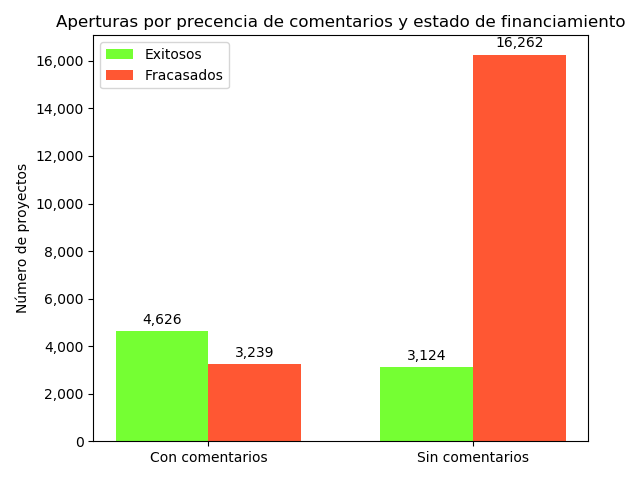
\includegraphics[width=0.80\textwidth]{4/figures/projects comment by state.png}
		\caption[Distribución de proyectos por presencia de comentarios y estado final]{Distribución de proyectos por presencia de comentarios y estado final.\\
			Fuente: Elaboración propia.}
		\label{4:fig24}
	\end{center}
\end{figure}

Esto señala que es más probable que un proyecto sin recibir comentarios tiende a fracasar por la diferencia notable entre ambas categorías (68\%). Por el contrario, para el caso de aquellos que presentan comentarios, no se puede formular una hipótesis sobre su comportamiento ya que la diferencia de proporciones no es muy alta (20\%) en comparación con el grupo sin comentarios. Por ello, para conocer un poco más a este último grupo, se analizó el impacto de las cantidades de comentarios independientes realizados por patrocinadores exclusivamente en el resultado final de la meta de financiamiento.

\newpage
De aquellos proyectos con comentarios, el 96\% que fueron financiados exitosamente recogieron más de 475 mil comentarios, como se aprecia en la Figura \ref{4:fig25}.

\begin{figure}[!ht]
	\begin{center}
		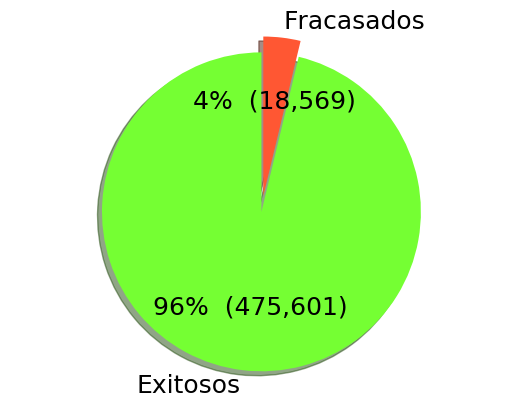
\includegraphics[width=0.44\textwidth]{4/figures/total comments by projects state.png}
		\caption[Distribución de comentarios en proyectos exitosos y fracasados]{Distribución de comentarios en proyectos exitosos y fracasados.\\
			Fuente: Elaboración propia.}
		\label{4:fig25}
	\end{center}
\end{figure}

Respecto al contenido, en la Figura \ref{4:fig26} se ilustra la nube de palabras más frecuentes, respectivamente, luego de quitar URLs, emoticonos y términos en idioma distinto al inglés.

\begin{figure}[htbp]
	\begin{center}
		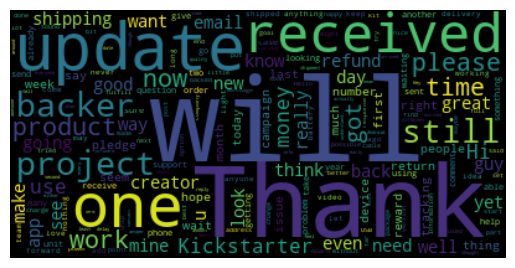
\includegraphics[width=0.68\textwidth]{4/figures/comments_wordcloud_wordunit.png}
		\caption[Nube de palabras de comentarios más frecuentes]{Nube de palabras de comentarios más frecuentes.\\
			Fuente: Elaboración propia.}
		\label{4:fig26}
	\end{center}
\end{figure}

De esta imagen, se observa que las palabras más frecuentes en los comentarios (tamaño de fuente más grande) se relacionan con términos clave respecto a la campaña (\textit{update}, \textit{project}, \textit{backer}, \textit{product} y \textit{Kickstarter}) y palabras relacionadas a su interacción con el público (\textit{thank}, \textit{will}, \textit{received}, \textit{time}, \textit{money}). Algunos de estos términos, tanto en su forma raíz como en conjugaciones, suelen aparecer solitarias o acompañados de otros para formar frases recurrentes.

\section{Preparación de los datos}
\textbf{Actividad 1: Pre-procesar base de datos de Metainformación}
\\
De acuerdo a los autores \cite{pr_chen2013kickpredict}, \cite{pr_chen2015predcrowd} y \cite{pr_jin2019dayssuccess}, a las 5 potenciales variables numéricas se adicionaron 7 variables basadas en el mecanismo financiero (mediana (\textit{pledges\_median}), promedio (\textit{pledges\_mean}), valor máximo (\textit{pledges\_max}), valor mínimo (\textit{pledges\_min}), variación estándar (\textit{pledges\_std}) y cantidad de montos disponibles para contribuir (\textit{pledges\_num})) y efecto progresión (porcentaje de financiamiento o completitud (\textit{completeness}) del monto prometido). Esta última se calcula dividiendo el monto alcanzado en el tiempo t, sobre la meta de la campaña, multiplicado por 100\%. La nueva matriz de correlación se observa en la Figura \ref{4:fig27}.

\begin{figure}[!ht]
	\begin{center}
		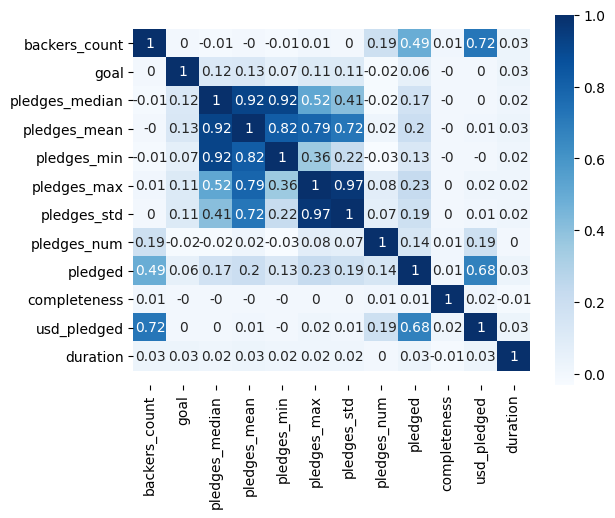
\includegraphics[width=1.00\textwidth]{4/figures/metadata correlation v2.png}
		\caption[Matriz de correlaciones entre variables independientes considerando adicionales]{Matriz de correlaciones entre variables independientes considerando adicionales.\\
			Fuente: Elaboración propia.}
		\label{4:fig27}
	\end{center}
\end{figure}

\newpage
Para la selección de variables, se consideró a aquellas con correlación clasificada como insignificante, es decir, menor o igual a 0.30 \parencite{tec_mukaka2012correlation}. Las únicas que cumplen son \textit{goal}, \textit{pledges\_num}, \textit{completeness} y \textit{duration}. Sin embargo, algunas de las restantes pueden ser consideradas condicionándose a excluir otras. En la Tabla \ref{4:table2} se listan las 8 combinatorias posibles de variables que se pueden formar.

\begin{table}[h!]
	\caption[Potenciales combinatorias de variables de metainformación]{Potenciales combinatorias de variables de metainformación.}
	\label{4:table2}
	\centering
	\small
	\begin{tabular}{ m{3.5cm}m{3.5cm}m{3.5cm}m{3.5cm}  }
		\specialrule{.1em}{.05em}{.05em}
		%\rowcolor{bluejean}
		\Centering{Combinación 1}& \Centering{Combinación 2}& \Centering{Combinación 3}& \Centering{Combinación 4}
		\\
		\specialrule{.1em}{.05em}{.05em}
		goal & goal & goal & goal \\
		\hline
		completeness & completeness & completeness & completeness
		\\
		\hline
		duration & duration & duration & duration
		\\
		\hline
		pledges\_num & pledges\_num & pledges\_num & pledges\_num
		\\
		\hline
		backers\_count & backers\_count & backers\_count & backers\_count \\
		\hline
		pledges\_median & pledges\_mean & pledges\_min & pledges\_max \\
		\hline
		&  & pledges\_std &  \\
		\specialrule{.1em}{.05em}{.05em}
		\Centering{Combinación 5}& \Centering{Combinación 6}&
		\Centering{Combinación 7}& \Centering{Combinación 8}
		\\
		\specialrule{.1em}{.05em}{.05em}
		goal & goal & goal & goal
		\\
		\hline
		completeness & completeness & completeness & completeness
		\\
		\hline
		duration & duration & duration & duration
		\\
		\hline
		pledges\_num & pledges\_num & pledges\_num & pledges\_num
		\\
		\hline
		pledged & pledged & pledged & pledged \\
		\hline
		pledges\_median & pledges\_mean & pledges\_min & pledges\_max \\
		\hline
		&  & pledges\_std &  \\
		\specialrule{.1em}{.05em}{.05em}
	\end{tabular}
	%\par	%%Salto de linea
	%\bigskip
	\begin{flushleft}	%%Alinear a la izquierda sin justificar
		\small Fuente: Elaboración propia.
	\end{flushleft}
\end{table}

Una vez generadas las variables independientes (X) y dependiente (Y), el conjunto de datos es separado en subconjuntos de entrenamiento y prueba, con proporciones de 80\% y 20\% respectivamente \citep{pr_yuan2016textanalytics,pr_yu2018deeplearning,pr_chen2019keywords_crowdfunding,pr_mitra2014phrases,pr_sawhney2016usingLT} y se fija un valor de aleatoriedad. Dentro de los parámetros de separación, se establece el argumento de estratificación según la variable Y, es decir, cada subconjunto mantendrá la distribución 72\% exitosos y 28\% fracasados.

\begin{figure}[!ht]
	\begin{center}
		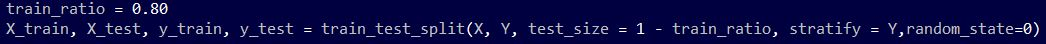
\includegraphics[width=1.00\textwidth]{4/figures/train_test_split.jpg}
		\caption[Función para dividir base de datos en subconjuntos de entrenamiento y prueba]{Función para dividir base de datos en subconjuntos de entrenamiento y prueba.\\
			Fuente: Elaboración propia.}
		\label{4:fig28}
	\end{center}
\end{figure}

Luego, utilizando el escalador Mínimo Máximo (\textit{Min-Max scaler}) de la librería Scikit-learn, se normalizaron las variables independientes a un nuevo rango conformando valores entre 0 y 1. La función creada para este proceso se muestra en la Figura \ref{4:fig29}.

\begin{figure}[!ht]
	\begin{center}
		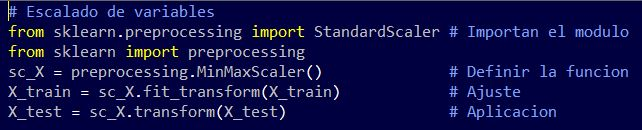
\includegraphics[width=0.95\textwidth]{4/figures/metadata_scaler_function.jpg}
		\caption[Función para normalizar variables]{Función para normalizar variables.\\
			Fuente: Elaboración propia.}
		\vspace{-0.5cm}
		\label{4:fig29}
	\end{center}
\end{figure}

Para calcular los nuevos valores normalizados usando el anterior escalador, se sigue la siguiente fórmula \citep{tec_minmaxscaler,tec_scikitlearn,tec_datascaling}:

\begin{equation}\label{eq:minmaxscaler}
\phantomsection
x_{escalado}=\frac{x-x_{min}}{x_{max}-x_{min}}
\end{equation}
\myequations{Fórmula del escalador Mínimo Máximo}

Donde $x$ representa el valor original de un dato, $x_{min}$ el valor mínimo existente para dicha variable y $x_{max}$, el valor máximo.

Por ejemplo, tomando como referencia las estadísticas de la variable \textit{duration} en la Figura \ref{4:fig19}, se desea transformar una duración de 30 días dentro del rango [0; 1]. Para aplicar la fórmula, los valores serían $x=30$, $x_{min}=1$ y $x_{max}=92$. Entonces, el nuevo resultado sería $x_{escalado}=\frac{30-1}{92-1}=0.32$.

\vspace{0.5cm}
\textbf{Actividad 2: Pre-procesar base de datos de Descripción}
\\
Se realizó la limpieza de texto basándose en los trabajos de los autores \cite{pr_mitra2014phrases}, \cite{pr_yuan2016textanalytics} y \cite{pr_chen2019keywords_crowdfunding} y además, se agregaron pasos de lematización y supresión de palabras de parada siguiendo el proceso dictado en el curso de Procesamiento de Lenguaje Natural en la Escuela Superior de Economía de la Universidad Nacional de Investigación, Rusia \parencite{tec_zimovnov2018text_preprocessing}. Antes de ejecutarse el proceso, los registros sin descripciones (\textit{NaN}) fueron convertidos en cadena (\textit{string}) para evitar problemas de procesamiento de texto. Se remueven las contracciones, caracteres especiales, enlaces externos y contenidos en otros idiomas. Este resultado fue separado en palabras o tókens para eliminar palabras de parada en inglés, lematizar las restantes y finalmente juntarlas en una lista por su proyecto.

Cada iteración se pudo lograr gracias a elementos de la biblioteca para procesamiento de lenguaje natural Natural Language Toolkit (NLTK), como por ejemplo \textit{word\_tokenize}, \textit{stopwords} y \textit{WordNetLemmatizer}. La descripción de mayor longitud pasó a presentar 3,671 palabras y a nivel general de proyectos, el nuevo vocabulario tuvo 165,526 palabras.

Las nubes de palabras reflejan las palabras más frecuente dentro de un conjunto de datos. La Figura \ref{4:fig30} representa aquellas palabras que más aparecen en las descripciones.

\begin{figure}[!ht]
	\begin{center}
		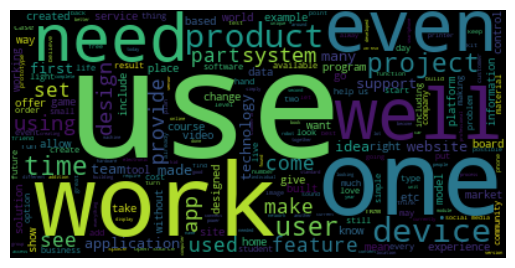
\includegraphics[width=0.65\textwidth]{4/figures/description_wordcloud.png}
		\caption[Nube de palabras de descripciones posterior a la limpieza de texto]{Nube de palabras de descripciones posterior a la limpieza de texto.\\
			Fuente: Elaboración propia.}
		\label{4:fig30}
	\end{center}
\end{figure}

Luego de la limpieza de textos, la variable independiente \textit{description}, como en el caso de Metainformación, fue dividida en subconjuntos de 80\% para entrenamiento y 20\% para prueba, estratificados según la distribución de la variable \textit{state}. A continuación, en la Figura \ref{4:fig31} se ejecuta el proceso para representar las palabras de las descripciones en vectores.

\begin{figure}[!ht]
	\begin{center}
		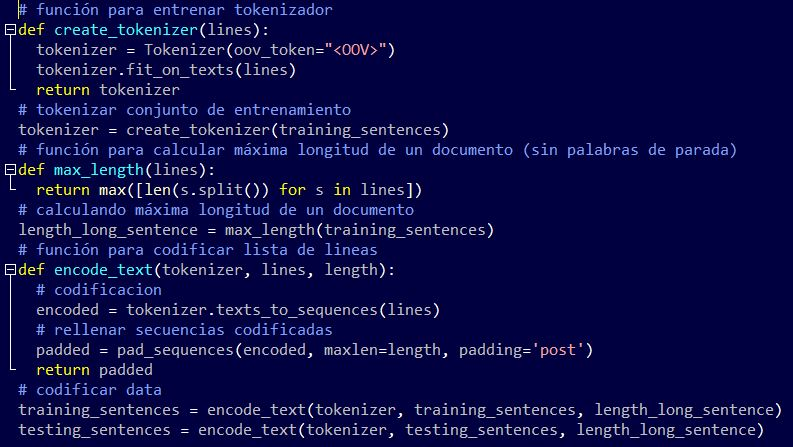
\includegraphics[width=0.95\textwidth]{4/figures/description_word_representation.jpg}
		\caption[Proceso de representación de palabras en vectores codificados]{Proceso de representación de palabras en vectores codificados.\\
			Fuente: Elaboración propia.}
		\label{4:fig31}
	\end{center}
\end{figure}

De acuerdo al algoritmo de la figura anterior, se usó la función \textit{Tokenizer} de la librería \textbf{tensorflow.keras.preprocessing.text}, para separar las palabras únicas o \textit{tokens} de una línea de texto asignada. En caso se encuentre un término no identificado dentro del diccionario a entrenar, se asignará a dicho token el valor de \textit{$<$OOV$>$}. Esta función se aplicó al subconjunto de entrenamiento para elaborar un diccionario a partir de sus tokens. Luego, se creó una función para determinar la mayor longitud de palabras de las descripciones del dataset. Esta cantidad representó 3,671 términos. A continuación, se desarrolló una función para crear una secuencia de las palabras codificadas, homologar hasta la máxima longitud de descripciones y rellenar con ceros a la derecha (parámetro \textit{padding=`post'}) en caso un vector no alcance esta longitud. Se aplicó este proceso a los subconjuntos originales de entrenamiento y prueba.

Una vez obtenido el vocabulario de palabras únicas y asignado el tamaño de cada arreglo (en este caso, se asignó el de la descripción de mayor longitud), se procedió a elaborar la matriz de características usando incrustaciones de GloVe como se observa en la Figura \ref{4:fig32}. Para la presente investigación, se seleccionó la opción Wikipedia 2014 + Gigaword 5, con una matriz de 100 columnas, donde cada una contendrá las incrustaciones de palabras GloVe para las palabras del corpus, cuyos índices se corresponderán con cada número de fila \parencite{tec_malik2019pythonnlp}.

\begin{figure}[!ht]
	\begin{center}
		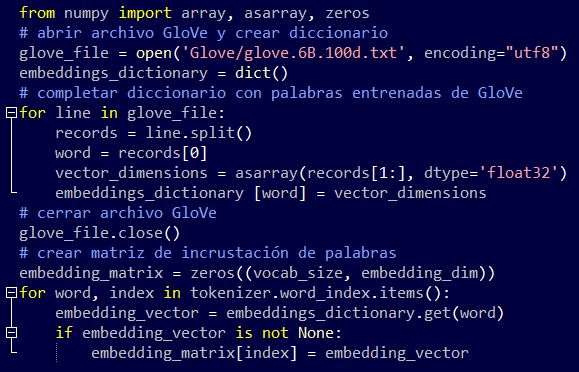
\includegraphics[width=0.75\textwidth]{4/figures/description_embedding_matrix.jpg}
		\caption[Proceso de creación de matriz de incrustaciones de palabras]{Proceso de creación de matriz de incrustaciones de palabras.\\
			Fuente: Elaboración propia.}
		\label{4:fig32}
	\end{center}
\end{figure}

En la figura anterior, luego de abrirse el archivo GloVe, se completa un diccionario creado con los registros extraídos del algoritmo GloVe. Luego de terminarse este proceso y cerrarse el archivo, se crea la matriz de incrustación de palabras que será utilizada más adelante en la capa de incrustación del modelo predictivo.

\textbf{Actividad 3: Pre-procesar base de datos de Comentarios}
\\
La base de datos de comentarios está conformada a nivel de 1 proyecto con una lista de comentarios separados en sublistas. De los 7,750 proyectos con comentarios (4,626 exitosos), se removieron aquellos que presentaron términos en idioma distinto al inglés, URLs, emoticonos, emojis, números y caracteres especiales, quedando 7,658 registros (4,574 exitosos).

Debido a la gran cantidad de registros carecientes de comentarios, se propuso rellenarlos con un término aleatorio no relacionado con las temáticas principales: \textit{kuwagatabaizan}. Posteriormente, se repitió el mismo ejercicio para las descripciones. Sin considerar este nuevo término, la nube de palabras se representa en la Figura \ref{4:fig33}.

\begin{figure}[!ht]
	\begin{center}
		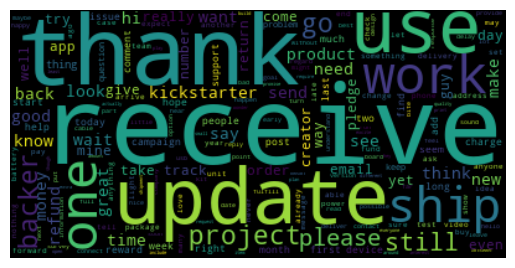
\includegraphics[width=0.63\textwidth]{4/figures/comments_wordcloud_processed.png}
		\caption[Nube de palabras de comentarios posterior a la limpieza de texto]{Nube de palabras de comentarios posterior a la limpieza de texto.\\
			Fuente: Elaboración propia.}
		\label{4:fig33}
	\end{center}
\end{figure}

Al igual que el caso de Descripción, se siguieron los procesos de la Figura \ref{4:fig31} para obtener la representación de palabras en vectores codificados y la Figura \ref{4:fig32} para crear la matriz de incrustación de palabras que se usarán en la capa de incrustaciones, con la diferencia en que el tamaño de la secuencia de palabras codificadas no será la máxima longitud de comentarios ya que estos, inicialmente separados por autor, al ser concatenados en un solo registro por proyecto, ampliaron su longitud exponencialmente. La máxima longitud de todos los registros fue de 30,072 palabras; por ello, se limitó el tamaño de secuencias a 5,000 términos.